\documentclass[8pt]{beamer}

% ---------- Theme ----------
\usetheme{Madrid}          % Other options: Berlin, Warsaw, default, Boadilla, CambridgeUS
\usecolortheme{default}    % Other options: beaver, dolphin, seahorse

% ---------- Packages ----------
\usepackage[utf8]{inputenc}
\usepackage{graphicx}
\usepackage{amsmath}
\usepackage{tikz}
\usetikzlibrary{decorations.pathreplacing}
\usepackage{hyperref}

% ---------- Title Page Info ----------
\title[Steganography with LLMs]{Unbreakable Steganography with LLMs}
% \subtitle{An Optional Subtitle}
\author{Stephan Wäldchen}
\institute{Iliad Intensive June 2026}
% \date{\today}

% ---------- Document ----------
\begin{document}

% Title slide
\begin{frame}
    \titlepage
\end{frame}

% Table of contents (optional)
\begin{frame}{Outline}
    \tableofcontents
\end{frame}

% ---------- Section 1 ----------
\section{Overview}

\begin{frame}{Steganography Setup}

    \begin{figure}
        
\includegraphics[width=0.6\textwidth]{fig/stego_schematic.png}
    \end{figure}

Ingredients:
    \begin{itemize}
        \item Sender/Encoder $E$ and Receiver/Decoder $D$
        \item Communication Channel $C$
        \item A secret key $k$ shared by $E$ and $D$
        \item A distribution $\mathcal{D}$ of innocent messages
        \item A message space $M$
    \end{itemize}
    
\end{frame}

\begin{frame}{Can we have perfect perfect information theoretic security?}

    \begin{figure}
        
\includegraphics[width=0.4\textwidth]{fig/Message_entropy.png}
    \end{figure}

Perfect Steganography:
\begin{itemize}
    \item M: Message, X: Stego-Text, K: Key
    \item Perfect Security: $I(M;X) = 0$
    \item Perfect Decoding: $H(M| X, K) = 0$
\end{itemize}

\begin{align}
    I(M;X,K) &= H(M) - H(M|X,K) & \quad \text{(Def of Mut. Info)} \\
    I(M;X,K) &= I(M ; X) + I(M;K|X) & \quad \text{(Chain Rule)} \\
    \Rightarrow H(M) &= \underbrace{H(M|X,K)}_{=0} + \underbrace{I(M ; X)}_{=0} + I(M;K|X) \leq H(K) \\
    \Rightarrow H(M) &\leq H(K)
\end{align}
\end{frame}




\begin{frame}{Computationally Secure Steganography}

\begin{itemize}
    \item Basic Idea: Security against polynomially bounded adversaries
    \item Uses Pseudo-Random Functions (PRF), i.e., deterministic functions
\[
F=\left\{
F_k:\{0,1\}^{|x|}\to\{0,1\}^{|y|}
\right\}_{k\in\{0,1\}^{|k|}},
\]
[ $|k|, |x|=\text{poly}(|k|), |y|=\text{poly}(|k|)$ are key, input and output length]
\item where, for any poly-time distinguisher $D$, the advantage
\[
\operatorname{Adv}^{\mathrm{PRF}}_{F,D}(|k|)
:=
\left|
\Pr_{k}
\left[
D^{F_k}(1^{|k|})=1
\right]
-
\Pr_{f}
\left[
D^{f}(1^{|k|})=1
\right]
\right|,
\]
where
\[
    k\sim\mathcal{U}\left(\{0,1\}^{|k|}\right) \quad \text{and}\quad
    f\sim\mathcal{U}\left(\{0,1\}^{|x|}\to\{0,1\}^{|y|}\right)
\]
is negligable, i.e., 
\[
\operatorname{Adv}^{\mathrm{PRF}}_{F,D}(|k|) < \frac{1}{\text{poly}(k)}
\]
\end{itemize}


\end{frame}

% ---------- Section 2 ----------
\section{Main Content}

\begin{frame}{PRF + LLM = Unbreakable Steganography}

    \begin{itemize}
        \item Any signal that has entropy (or random degrees of freedom), can be turned into an unbreakable stego scheme via PRFs
        \item Basic Idea:
        \begin{itemize}
            \item Sender and Receiver share PRF scheme and secret key $k$
            \item Sender uses LLM to generate distribution over next token
            \item The PRF with the next symbol as input generates a pseudo-random sample
            \item The receiver eliminates every symbol that wasn't compatible with the tokens so far until only one symbol remains
            \item Sender moves on to next symbol
        \end{itemize}
    \end{itemize}


\begin{figure}
    \centering
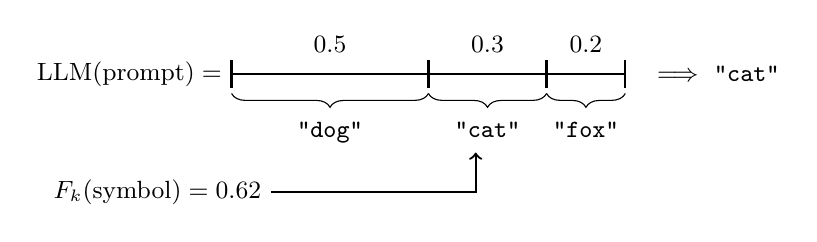
\begin{tikzpicture}[
    x=0.5cm,
    y=1cm,
    font=\small,
    tokenbrace/.style={
        decorate,
        decoration={
            brace,
            mirror,
            amplitude=5pt
        }
    }
]

% Main probability interval
\draw[thick] (0,0) -- (10,0);

% Tick marks
\foreach \x in {0,5,8,10}
    \draw[thick] (\x,-0.18) -- (\x,0.18);

% Probabilities
\node[above=4pt] at (2.5,0) {$0.5$};
\node[above=4pt] at (6.5,0) {$0.3$};
\node[above=4pt] at (9,0) {$0.2$};

% Three downward-pointing braces
\draw[tokenbrace] (0,-0.25) -- (5,-0.25)
    node[midway,below=7pt] {\texttt{"dog"}};

\draw[tokenbrace] (5,-0.25) -- (8,-0.25)
    node[midway,below=7pt] {\texttt{"cat"}};

\draw[tokenbrace] (8,-0.25) -- (10,-0.25)
    node[midway,below=7pt] {\texttt{"fox"}};

% LLM label
% LLM label
\node[anchor=east] at (0,0)
    {$\mathrm{LLM}(\mathrm{prompt}) =$};

% PRF value, aligned equally far left
\node[anchor=east] at (1,-1.5)
    {$F_k(\mathrm{symbol})=0.62$};
\draw[thick,->]
    (1,-1.5) -- (6.2,-1.5) -- (6.2,-1.0);

% Selected output
\node[right=8pt] at (10,0)
    {$\Longrightarrow\ \texttt{"cat"}$};

\end{tikzpicture}
    \caption{Using a PRF to select from the next-token distribution}
    \label{fig:placeholder}
\end{figure}
    
\end{frame}

\begin{frame}{Error Correction}
    
    \begin{itemize}
        \item \textbf{Scenario 1:} LLM and prompt are known $\rightarrow$. Receiver can decode perfectly
        \item \textbf{Scenario 2:} Only tokenizer is known: Receiver can still decode probabilistically with error correction ($\leftarrow$ symbol)
        \item Receiver aggregates score for every symbol 
        \item Once score exceeds threshold $t$, symbol is accepted
        \item If a wrong symbol got accepted, the sender sends a $\leftarrow$ correction symbol
        \item As long as the error rate is $<0.5$, the process has net progress towards correct symbols
    \end{itemize}

    
\end{frame}

\begin{frame}
    \centering
    \Huge Questions?
\end{frame}

\end{document}